\chapter{AI in Prototyping: Capability \& Risk}
\label{ch8}

\paragraph{Where this fits.}
This chapter operates at Stage~3 (Development) of the Stage-Gate model.
AI tools are increasingly present inside Stage~3 design work --- generating
firmware scaffolding, suggesting component values, exploring design alternatives,
and drafting documentation.
Every AI output that enters your design must be verified before it becomes
Gate~3 evidence; this chapter gives you the framework to decide what to verify,
how rigorously, and how to document it.

\paragraph{Learning Objectives.}
After completing this chapter, you will be able to:
\begin{enumerate}
  \item Identify three categories of design task where AI tools provide
        genuine value in the prototyping workflow.
  \item Compute the expected cost of error for an AI-generated output and
        apply the verification decision rule to determine whether independent
        verification is required before incorporating the output into a design.
  \item Assess the IP and data-leakage risk of using a public AI tool with
        proprietary design data and identify at least two specific categories
        of Stage~3 information that must not be submitted to a public service
        without checking the provider's retention policy.
  \item Document AI use in a reproducible, traceable format suitable for a
        Gate~3 submission.
\end{enumerate}

Chapter~7 delivered a component-verified, assembly-optimised, test-instrumented
schematic package ready for Gate~3 review --- produced by applying four DFX
frameworks to the Stage~3 design.
It did not address the AI tools many teams reach for inside that same stage to
accelerate the work.
This chapter provides the framework for using those tools without compromising
the integrity of the design package.

% ─────────────────────────────────────────────────────────────────────────────
\section{Where AI Helps}
\label{sec:ch8-helps}
% ─────────────────────────────────────────────────────────────────────────────

\textbf{AI-assisted design}\index{AI-assisted design} tools --- large-language
models, code-completion engines, and component-suggestion services --- can
reduce the time spent on routine, well-defined sub-tasks within Stage~3.
Three categories of task account for most of the practical value in a
prototyping workflow.

\subsection{Code and Firmware Scaffolding}
\label{sec:ch8-helps-code}

Writing peripheral initialisation code, interrupt handlers, communication
protocol wrappers, and RTOS task skeletons is repetitive and follows patterns
that are well-represented in publicly available firmware.
An AI tool can generate a working first draft of a UART driver, an I$^2$C
read/write wrapper, or a timer-interrupt handler in seconds.

The value is not that the output is correct by default --- it often is not, for
reasons discussed in Section~\ref{sec:ch8-hallucination}.
The value is that a plausible first draft is faster to correct than to write
from scratch, and it forces the engineer to think through the design at the
code level earlier in the process.

For the running-example sorter project, AI-generated firmware scaffolding is
useful for the sort-accuracy inference pipeline: the AI can produce a skeleton
that reads sensor data, formats it for the inference engine, and routes the
classification result to the conveyor control loop.
The engineer then verifies each section against the MCU datasheet and the
inference engine's API specification.

\subsection{Component Value Suggestion}
\label{sec:ch8-helps-component}

Selecting passive component values --- pull-up and pull-down resistors,
decoupling capacitors, RC filter time constants --- requires applying well-known
formulas to circuit-specific parameters.
An AI tool can propose a value given a natural-language description of the
circuit context (``10 kHz I$^2$C bus, 400 pF estimated bus capacitance'').

The suggestion reduces search time.
It does not replace the engineer's obligation to verify the value against the
datasheet application note and, where relevant, to bench-test the result.
Section~\ref{sec:ch8-blackbox} establishes when bench verification is required.

\subsection{Design Alternatives and Documentation Drafts}
\label{sec:ch8-helps-docs}

AI tools can enumerate design alternatives quickly: given a power-supply
topology requirement, they can list candidate topologies with broad trade-offs.
This is useful for early-stage exploration, where breadth matters more than
depth.
The engineer evaluates the shortlist using the selection criteria from
Chapter~6, not the AI's ranking.

AI tools also accelerate documentation drafts: block-diagram descriptions,
BOM notes, test-procedure outlines, and design-rationale summaries can all be
drafted from a structured prompt and then edited for accuracy and completeness.
Documentation drafted by AI must be reviewed against the actual design
before submission; Chapter~9 will show why incomplete or inaccurate
safety documentation has consequences beyond a Gate~3 review.

% ─────────────────────────────────────────────────────────────────────────────
\section{Accelerator, Not Autonomous Designer}
\label{sec:ch8-accelerator}
% ─────────────────────────────────────────────────────────────────────────────

One principle governs all AI-assisted design work: \textbf{the engineer is
accountable for every output that enters the design}\index{engineer accountability},
regardless of how that output was produced.

An AI tool has no professional licence, no liability, and no understanding of
your specific circuit, budget, safety obligations, or regulatory context.
It produces plausible text and code based on statistical patterns in its
training data.
When that output happens to be correct, it saves time.
When it is wrong --- and it will be wrong, in ways described in
Section~\ref{sec:ch8-hallucination} --- the engineer who accepted it without
verification is responsible for the consequence.

This is not a philosophical position; it has direct implications for Gate~3 evidence.
A Gate~3 review asks: ``How do you know this design meets specification?''
``The AI said so'' is not an answer that survives scrutiny.
``The AI suggested it; we verified it by \emph{[method]}; the result was
\emph{[outcome]}'' is.

\textbf{Design acceleration}\index{design acceleration} is the correct mental
model for AI in Stage~3.
An AI tool does not change what must be verified or who must verify it; it
changes how long the first draft takes to produce.

% ─────────────────────────────────────────────────────────────────────────────
\section{Hallucination in an Engineering Context}
\label{sec:ch8-hallucination}
% ─────────────────────────────────────────────────────────────────────────────

\textbf{AI hallucination}\index{AI hallucination} is a specific failure mode
distinct from a simple factual error.
A factual error is a wrong answer to a question that has a right answer in the
AI's training data --- the AI retrieves the wrong datum.
A hallucination is a confidently stated answer that has no factual basis at
all: the AI generates a plausible-sounding output that does not correspond to
any real specification, component, or physical relationship.

In an engineering context, hallucinations are more dangerous than factual
errors for one reason: \emph{they look right}.
A factual error --- a resistor value that is obviously wrong for the voltage
level --- is caught by inspection.
A hallucination --- a pull-up resistor value that is plausible for many buses
but wrong for this specific bus speed and capacitive load --- passes visual
inspection and may even pass a basic functional test, failing only under the
exact operating conditions of your application.

\subsection{The Human-in-the-Loop Verification Cycle}
\label{sec:ch8-hitl}

The response to hallucination risk is a structured
\textbf{human-in-the-loop (HITL) verification cycle}\index{human-in-the-loop
verification}.
Figure~\ref{fig:ch8-hitl} shows the cycle.

\begin{figure}[htbp]
  \centering
  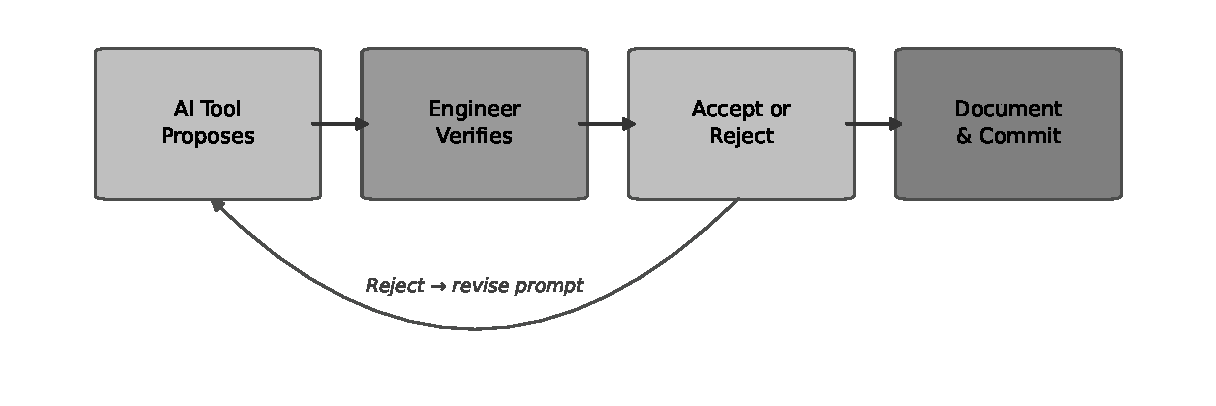
\includegraphics[width=0.85\textwidth]{images/fig_01_hitl_loop}
  \caption{The human-in-the-loop verification cycle for AI-generated design
           outputs. The engineer generates a candidate output using an AI tool,
           applies an independent verification method (datasheet check,
           simulation, bench test, or first-principles calculation), and either
           accepts the output and logs it, or rejects it and either regenerates
           or derives the value manually. The cycle is not optional; it applies
           to every AI output that enters the design.}
  \label{fig:ch8-hitl}
\end{figure}

The cycle has four steps:
\begin{enumerate}
  \item \textbf{Generate.} Prompt the AI tool with enough context to produce a
        specific, actionable output.
        Vague prompts produce vague outputs; vague outputs are harder to verify.
  \item \textbf{Estimate risk.} Assign a probability of error $p_{\text{err}}$
        and a consequence cost $C_{\text{consequence}}$ to the output.
        Section~\ref{sec:ch8-blackbox} shows how to use these to decide
        verification depth.
  \item \textbf{Verify independently.} Apply a verification method that is
        independent of the AI tool: datasheet application note, SPICE
        simulation, analytical calculation, or bench measurement.
  \item \textbf{Accept or reject and log.} Record what the AI produced, how
        it was verified, and the result.
        Section~\ref{sec:ch8-traceability} specifies the log format.
\end{enumerate}

\paragraph{In Practice.}
A first-principles priority review of AI-generated interrupt handlers can catch
failures that functional tests miss, as the following example illustrates.
A team used AI to generate firmware interrupt handlers for a real-time
scheduler on the running-example sorter.
The AI output compiled cleanly and passed basic unit tests.
The interrupt handler correctly serviced the conveyor-belt encoder pulses at
low throughput.
Under the 6~items/min throughput target, however, interrupt latency spiked
intermittently and caused missed encoder edges.
Root-cause analysis identified a race condition in the interrupt priority
scheme: the AI had assigned equal priority to the encoder interrupt and a
lower-frequency status-reporting interrupt.
When status reporting and an encoder pulse arrived simultaneously at high
throughput, the encoder pulse was occasionally delayed by the status-reporting
ISR.
A first-principles review of the interrupt priority assignment --- checking
each interrupt against the real-time deadline table in the design specification
--- caught the race condition before deployment.
The fix was a one-line priority change; the cost of not catching it would have
been a throughput failure at Gate~3 demonstration.

% ─────────────────────────────────────────────────────────────────────────────
\section{The Black-Box Problem: Deciding When to Verify}
\label{sec:ch8-blackbox}
% ─────────────────────────────────────────────────────────────────────────────

You cannot always verify every AI output at the same depth: bench testing
every component value is not feasible in a constrained schedule.
A quantitative decision rule prevents both under-verification (trusting
plausible output that is wrong) and over-verification (spending verification
time that exceeds the value at risk).

\subsection{Expected Cost of Error}
\label{sec:ch8-expected-cost}

The \textbf{expected cost of error}\index{expected cost of error}
$\mathbb{E}[C_{\text{err}}]$ is:
%
\begin{equation}
  \label{eq:ch8-expected-cost}
  \mathbb{E}[C_{\text{err}}] = p_{\text{err}} \cdot C_{\text{consequence}}
\end{equation}
%
where $p_{\text{err}}$ is your estimated probability that the AI output is
wrong for your specific application, and $C_{\text{consequence}}$ is the
cost you will incur if the error reaches the prototype undetected (diagnosis
time, rework, schedule slip, or safety consequence).

The \textbf{verification decision rule}\index{verification decision rule} is:
\begin{quote}
  If $\mathbb{E}[C_{\text{err}}] > \text{cost\_verify}$, verify.
\end{quote}

This rule makes the verification decision quantitative and defensible.
It also reveals when verification is not cost-justified --- when the
consequence of a wrong value is trivially correctable and the verification
cost is disproportionate.
For safety-relevant functions, $C_{\text{consequence}}$ is large by definition,
and the rule will always recommend verification.

Figure~\ref{fig:ch8-trust} shows a trust matrix that maps AI output categories
against typical verification requirements.

\begin{figure}[htbp]
  \centering
  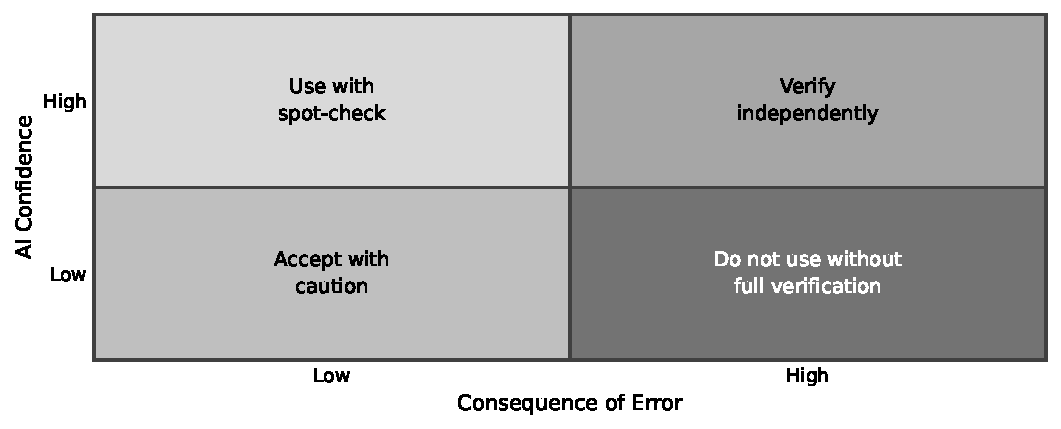
\includegraphics[width=0.85\textwidth]{images/fig_02_trust_matrix}
  \caption{Trust matrix for AI-generated design outputs. Outputs with low
           consequence cost and high AI reliability (e.g., boilerplate file
           structure, documentation phrasing) can be accepted with a visual
           review. Outputs with high consequence cost or low AI reliability
           (e.g., interrupt priority assignments, power-supply compensation
           networks, safety-critical logic) require independent simulation or
           bench verification before acceptance. No AI output to a safety-relevant
           function may be deployed unverified.}
  \label{fig:ch8-trust}
\end{figure}

\subsection{Worked Example: I\textsuperscript{2}C Pull-Up Resistor}
\label{sec:ch8-worked}

The running-example MCU board uses an I$^2$C bus to communicate with the sort
classifier's sensor array.
An AI tool suggests a 10~k$\Omega$ pull-up resistor for the bus.

The engineer's assessment:
\begin{itemize}
  \item $p_{\text{err}} = 0.15$: a 15\,\% chance the value is wrong for this
        bus speed (400~kHz fast mode) and the estimated 250~pF capacitive load
        of four sensors on a 15~cm trace.
        The I$^2$C specification limits the RC rise time, and at 400~kHz the
        bus capacitance matters; the AI did not have this context.
  \item $C_{\text{consequence}} = \$480$~CAD: one day of technician time to
        diagnose intermittent I$^2$C failures, identify the pull-up value as
        the cause, replace the resistor, and re-verify communication.
  \item $\text{cost\_verify} = \$40$~CAD: 20~minutes of engineer time to
        apply the I$^2$C pull-up selection equation from the NXP UM10204
        application note and check the result against a SPICE simulation of
        the bus topology.
\end{itemize}

Applying Equation~\ref{eq:ch8-expected-cost}:
\[
  \mathbb{E}[C_{\text{err}}] = 0.15 \times \$480 = \$72~\text{CAD}
\]

Decision: $\$72 > \$40$, so verification is justified.

The engineer applies the rise-time equation from the application note.
For a 400~kHz bus with $C_b = 250$~pF, the I$^2$C fast-mode specification
sets a maximum rise time $t_r = 300$~ns (NXP UM10204, Table~10).
The pull-up rise-time equation from that application note is:
\[
  R_{\max} = \frac{t_r}{0.8473 \cdot C_b}
\]
where the constant 0.8473 comes from the I$^2$C voltage threshold definition
($V_{\text{IH,min}} = 0.7\,V_{DD}$, giving $\ln(1/0.3)^{-1} \approx 0.8473$).
Substituting:
\[
  R_{\max} = \frac{300\,\text{ns}}{0.8473 \times 250\,\text{pF}}
           \approx 1{,}416\,\Omega
\]
The AI-suggested 10~k$\Omega$ would produce a rise time of approximately
2.1~$\mu$s --- seven times the I$^2$C fast-mode limit.
The AI output is rejected.
The engineer selects 1.0~k$\Omega$ (well within the $1{,}416\,\Omega$ maximum),
verifies the rise time is within specification, and logs the interaction.
Table~\ref{tab:ch8-worked-log} shows the complete AI use log entry for this
interaction; it satisfies the format specified in Section~\ref{sec:ch8-log}.

This is the HITL cycle in action: the AI output was plausible (10~k$\Omega$
is correct for standard-mode I$^2$C) but wrong for the specific operating
conditions.
The 20-minute verification prevented an intermittent bus failure that would
have been expensive to diagnose on a completed board.

\begin{table}[htbp]
  \centering
  \caption{AI use log entry for the I$^2$C pull-up resistor interaction.}
  \label{tab:ch8-worked-log}
  \small
  \begin{tabular}{@{}lp{0.72\textwidth}@{}}
    \toprule
    \textbf{Field} & \textbf{Entry} \\
    \midrule
    Tool used        & [AI service], accessed [date] \\
    Prompt summary   & Pull-up resistor value for 400~kHz I$^2$C bus,
                       $\approx$250~pF bus capacitance, four sensors on 15~cm trace. \\
    Output produced  & AI suggested 10~k$\Omega$. \\
    Verification     & NXP UM10204 rise-time equation; SPICE simulation of bus topology. \\
    Result           & \textbf{Rejected.} $R_{\max} \approx 1{,}416\,\Omega$ for fast
                       mode; selected 1.0~k$\Omega$. \\
    $\mathbb{E}[C_{\text{err}}]$ & $0.15 \times \$480 = \$72~\text{CAD} > \$40$
                       cost\_verify; verification justified. \\
    \bottomrule
  \end{tabular}
\end{table}

\paragraph{Common Pitfalls.}
Trusting plausible output without verification is the most common failure mode
when teams begin using AI tools in design work.
``It looked right'' is not an engineering justification.
An output that looks right for the general case is frequently wrong for your
specific combination of bus speed, supply voltage, load capacitance, and PCB
parasitics.

% ─────────────────────────────────────────────────────────────────────────────
\section{IP and Data-Leakage Risk}
\label{sec:ch8-ip}
% ─────────────────────────────────────────────────────────────────────────────

Using a public AI tool for design work introduces a risk that has no analogue
in traditional design tools: the data you submit may leave your control.

\subsection{What Happens to Your Data}
\label{sec:ch8-ip-data}

Public AI services vary widely in their data-retention policies.
Many services retain submitted content for model-improvement purposes unless
you explicitly opt out --- and the opt-out mechanism may not apply retroactively
to data already submitted.
Some services retain conversation history on their servers indefinitely.
Enterprise tiers with contractual data-handling guarantees exist, but they
require a procurement decision and are not the default for a student or small
team logging into a public web interface.

\textbf{Proprietary design data}\index{proprietary design data} submitted to a
public AI tool may therefore:
\begin{itemize}
  \item Be stored on the provider's servers beyond the session.
  \item Be used to train or fine-tune future model versions.
  \item Be retrievable, in whole or in part, through prompts from other users
        if it becomes embedded in model weights or cached session data.
  \item Constitute a public disclosure that affects patent-filing timelines in
        jurisdictions that require novelty.
\end{itemize}

\textbf{Data leakage}\index{data leakage} in this context does not require a
security breach.
It occurs through normal use of a service whose terms permit the provider to
use submitted content.

\subsection{What Constitutes Proprietary Data}
\label{sec:ch8-ip-what}

In a Stage~3 prototype context, the following are typically proprietary:
\begin{itemize}
  \item Schematics and PCB layouts that embody design decisions not yet in a
        granted patent or published application.
  \item Firmware source code, particularly inference-engine integration code
        that represents a competitive advantage.
  \item BOM entries that reveal supplier relationships or negotiated pricing.
  \item Design specifications that disclose performance targets ahead of a
        product announcement.
\end{itemize}

Generic questions --- ``what is the I$^2$C fast-mode maximum pull-up resistance
for 250~pF bus capacitance?'' --- carry no proprietary content.
Questions that include a schematic image, a firmware file, or project-specific
parameters that identify your design carry significant risk.

\paragraph{In Practice.}
A team pasted a proprietary motor-driver schematic into a public AI chat
session to ask for a component suggestion.
The schematic included part numbers, supplier codes, and a circuit topology
that was not yet in the prior art.
Six months later, when another user asked a similar question about motor-driver
design, the AI reproduced elements of the schematic --- part numbers and
a recognisable sub-circuit --- in its response.
The team had not read the provider's data-retention terms before submitting
the schematic; those terms permitted the provider to use submitted content
for model improvement.
The incident triggered a review by the organisation's legal counsel and
delayed a patent filing.

\subsection{The Data-Handling Policy}
\label{sec:ch8-ip-policy}

Before using any AI tool with design data, establish a simple policy:
\begin{enumerate}
  \item \textbf{Classify the data.} Is it generic (publicly available physics
        and formulas) or proprietary (specific to your design)?
  \item \textbf{Check the provider's terms.} Does the provider retain submitted
        content? Is there an enterprise or confidentiality tier?
  \item \textbf{Anonymise where possible.} Replace specific part numbers with
        generic descriptions; replace project-specific values with ranges.
        ``A pull-up resistor on a 400~kHz I$^2$C bus with 250~pF load'' reveals
        nothing proprietary. A schematic image does.
  \item \textbf{Log what was submitted.} The AI use log
        (Section~\ref{sec:ch8-traceability}) records a \emph{prompt summary},
        not the raw prompt, specifically to avoid logging proprietary data in a
        document that may be shared.
\end{enumerate}

\paragraph{Common Pitfalls.}
Submitting confidential design data to a public AI tool without checking the
provider's data-retention policy is a data-governance failure, not a technical
one.
The circuit may be correctly analysed; the design may be accelerated.
The risk is not to this prototype --- it is to every future product, patent
filing, or competitive position that depends on the information remaining
confidential.
Check the terms before you paste the schematic.

% ─────────────────────────────────────────────────────────────────────────────
\section{Reproducibility and Traceability}
\label{sec:ch8-traceability}
% ─────────────────────────────────────────────────────────────────────────────

Gate~3 requires evidence that your design decisions are defensible.
If AI tools contributed to a design decision, the Gate~3 record must show:
what the AI produced, how it was verified, and what the engineer decided as a
result.
A design whose AI contributions are undocumented cannot be reproduced,
audited, or defended.

\subsection{The AI Use Log}
\label{sec:ch8-log}

Every AI-assisted design interaction should produce an entry in an
\textbf{AI use log}\index{AI use log}.
Each entry contains:
\begin{enumerate}
  \item \textbf{Tool used.} Name and version (or access date) of the AI
        service.
  \item \textbf{Prompt summary.} A description of what was asked, with no
        proprietary data.
        Example: ``Asked for pull-up resistor value for 400~kHz I$^2$C bus
        with approximately 250~pF capacitive load.''
  \item \textbf{Output produced.} The AI's specific recommendation.
        Example: ``AI suggested 10~k$\Omega$.''
  \item \textbf{Verification method.} How the output was checked.
        Example: ``Applied NXP UM10204 rise-time equation; SPICE simulation of
        bus topology.''
  \item \textbf{Result.} Accepted or rejected, with brief rationale.
        Example: ``Rejected. Calculated $R_{\max} \approx 1{,}416\,\Omega$ for
        fast mode; selected 1.0~k$\Omega$.''
  \item \textbf{$\mathbb{E}[C_{\text{err}}]$ computed.} The expected cost of
        error used to justify the verification decision.
\end{enumerate}

A log entry takes less than five minutes to write.
It transforms an undocumented shortcut into a traceable, auditable design
decision.

\paragraph{Common Pitfalls.}
The most consequential documentation failure is having no record of AI
involvement in a design.
If a Gate~3 reviewer asks ``How was this pull-up value selected?'' and the
answer is ``I asked an AI,'' the follow-up question is immediate: ``How was
the AI output verified?''
Without a log entry, you cannot answer that question.
With a log entry showing $\mathbb{E}[C_{\text{err}}] = \$72$ and verification
cost $= \$40$, and a rejection of the AI's suggestion with the correct value
derived from the application note, you have demonstrated exactly the engineering
judgment a Gate~3 review is designed to find.

\subsection{Reproducibility Requirement}
\label{sec:ch8-reproducibility}

\textbf{Reproducibility}\index{reproducibility} in this context means that a
second engineer reading the AI use log can reconstruct the verification
independently and reach the same conclusion.
Each log entry must be specific enough that a second engineer can reconstruct
the verification using the prompt summary, output record, named source, and
result fields specified in Section~\ref{sec:ch8-log}.

Reproducibility is not a bureaucratic requirement.
It is the standard of evidence that distinguishes engineering from guessing.

% ─────────────────────────────────────────────────────────────────────────────
\section*{Try It Yourself}
\addcontentsline{toc}{section}{Try It Yourself}
% ─────────────────────────────────────────────────────────────────────────────

A team uses AI to suggest a decoupling capacitor value for the 3.3~V power pin
of the MCU on the running-example sorter board.

\begin{itemize}
  \item $p_{\text{err}} = 0.20$: a 20\,\% chance the suggested value is
        suboptimal for this PCB layout (high-frequency bypass inadequate for
        the MCU's transient current demand).
  \item $C_{\text{consequence}} = \$600$~CAD: one day of debug and rework if
        the MCU resets intermittently under load at high throughput.
  \item $\text{cost\_verify} = \$25$~CAD: 15~minutes to check the MCU
        datasheet application note for the recommended decoupling network.
\end{itemize}

\begin{enumerate}
  \item[(a)] Compute $\mathbb{E}[C_{\text{err}}]$ using
             Equation~\ref{eq:ch8-expected-cost}.
  \item[(b)] Is verification justified? State the decision rule explicitly.
  \item[(c)] The team reduces $p_{\text{err}}$ to 0.04 by first checking the
             MCU datasheet application note before querying the AI, so the AI
             prompt includes the datasheet-recommended value range and asks
             only whether the layout parasitics would change the recommendation.
             Recompute $\mathbb{E}[C_{\text{err}}]$ and state whether
             verification is still justified.
  \item[(d)] \textit{(Conceptual)} Name two pieces of information that must
             appear in the AI use log entry for this interaction, beyond the
             tool name and date, and explain in one sentence why each is
             necessary for Gate~3 traceability.
\end{enumerate}

\noindent(No answer key provided.)

% ─────────────────────────────────────────────────────────────────────────────
\section*{Review Questions}
\addcontentsline{toc}{section}{Review Questions}
% ─────────────────────────────────────────────────────────────────────────────

\begin{enumerate}

  \item \textbf{(Conceptual)} List the three categories of design task from
  Section~\ref{sec:ch8-helps} where AI provides genuine value in the
  prototyping workflow.
  For each category, state one specific task from the running-example IoT
  robotic sorter project that falls within it.

  \item \textbf{(Conceptual)} Explain the difference between a factual error
  and an AI hallucination in an engineering context.
  Why is an AI hallucination potentially more dangerous than a simple factual
  error when it appears in a design output such as a component value or a
  firmware interrupt priority assignment?

  \item \textbf{(Applied --- calculation)} A team generates an AI-suggested
  motor-driver current-sense resistor value.
  The engineer estimates $p_{\text{err}} = 0.08$ and
  $C_{\text{consequence}} = \$1{,}200$~CAD (motor overcurrent damage and board
  replacement if the sense resistor is wrong).
  Bench verification of the value takes 30~minutes, equivalent to
  $\text{cost\_verify} = \$60$~CAD.
  \begin{enumerate}
    \item[(a)] Compute $\mathbb{E}[C_{\text{err}}]$ using
               Equation~\ref{eq:ch8-expected-cost}.
    \item[(b)] Is verification justified? Apply the decision rule explicitly.
    \item[(c)] At what value of $p_{\text{err}}$ does $\mathbb{E}[C_{\text{err}}]$
               exactly equal $\text{cost\_verify}$?
               Show the algebra.
               Then state: if the engineer could reduce $p_{\text{err}}$ to
               half the breakeven value by spending an additional \$15~CAD on
               a datasheet review before prompting the AI, is that additional
               expenditure cost-justified? Show your reasoning.
  \end{enumerate}

  \item \textbf{(Applied --- multi-step)} A team generates three AI outputs
  in one design session:
  \begin{itemize}
    \item Output~A: a pull-up resistor value.
          $p_{\text{err}} = 0.12$, $C_{\text{consequence}} = \$320$~CAD,
          $\text{cost\_verify} = \$30$~CAD.
    \item Output~B: a firmware loop structure for the conveyor control task.
          $p_{\text{err}} = 0.25$, $C_{\text{consequence}} = \$800$~CAD,
          $\text{cost\_verify} = \$50$~CAD.
    \item Output~C: a BOM line-item description for a passive component.
          $p_{\text{err}} = 0.05$, $C_{\text{consequence}} = \$80$~CAD,
          $\text{cost\_verify} = \$20$~CAD.
  \end{itemize}
  \begin{enumerate}
    \item[(a)] Compute $\mathbb{E}[C_{\text{err}}]$ for each output using
               Equation~\ref{eq:ch8-expected-cost}.
    \item[(b)] Which outputs should be verified according to the decision rule?
    \item[(c)] Rank \textbf{all three} outputs by verification priority
               (highest $\mathbb{E}[C_{\text{err}}]$ first), then identify
               the threshold $\mathbb{E}[C_{\text{err}}]$ value below which
               an output in this session would not justify verification.
  \end{enumerate}

  \item \textbf{(Conceptual)} A team member proposes submitting the following
  information to a public AI chat service to get component suggestions:
  a 48~V motor-driver schematic showing the full H-bridge topology, the
  project's part number prefix, and the target current rating.
  Using the data classification policy from Section~\ref{sec:ch8-ip-policy},
  identify which elements of this submission carry proprietary risk and state
  what anonymised substitution should be made for each before the prompt is
  submitted.

  \item \textbf{(Conceptual)} A colleague argues: ``We should just verify
  everything AI produces, so we never need to compute
  $\mathbb{E}[C_{\text{err}}]$.''
  Explain in two sentences why this policy fails in practice for a team
  operating under a fixed Stage~3 schedule.

\end{enumerate}

% ─────────────────────────────────────────────────────────────────────────────
\section*{End-of-Chapter Artifact}
\addcontentsline{toc}{section}{End-of-Chapter Artifact}
\label{sec:ch8-artifact}
% ─────────────────────────────────────────────────────────────────────────────

Produce an AI use log with at least three entries from your prototype design
session.
Each entry must include:
\begin{enumerate}
  \item \textbf{Tool used} --- name and version or access date.
  \item \textbf{Prompt summary} --- what was asked, with no proprietary data
        in the record.
  \item \textbf{Output produced} --- the specific value, code, or recommendation
        the AI returned.
  \item \textbf{Verification method applied} --- the independent check used
        (datasheet section, simulation, calculation, bench test).
  \item \textbf{Result} --- accepted or rejected, with the accepted or
        corrected value if rejected.
  \item \textbf{$\mathbb{E}[C_{\text{err}}]$ computed} --- the expected cost
        of error that justified the verification depth.
\end{enumerate}

At least one entry must result in a rejection (the AI output was wrong and a
corrected value was derived independently).

% ─────────────────────────────────────────────────────────────────────────────
\section*{Chapter Summary}
\addcontentsline{toc}{section}{Chapter Summary}
\label{sec:ch8-summary}
% ─────────────────────────────────────────────────────────────────────────────

AI tools accelerate Stage~3 design work in three categories: code and firmware
scaffolding, component value suggestion, and design alternatives and
documentation drafting.
In every category, the engineer remains the accountable party; AI provides a
faster first draft, not a substitute for independent verification.

The expected cost of error $\mathbb{E}[C_{\text{err}}] = p_{\text{err}} \cdot
C_{\text{consequence}}$ (Equation~\ref{eq:ch8-expected-cost}) makes the
verification decision quantitative: verify when $\mathbb{E}[C_{\text{err}}]$
exceeds the cost of verification.
The human-in-the-loop cycle (Figure~\ref{fig:ch8-hitl}) and the trust matrix
(Figure~\ref{fig:ch8-trust}) provide the operational framework for applying
this rule consistently.

IP and data-leakage risk requires a data-handling policy before AI tools are
used with design data: classify the data, check the provider's retention terms,
and anonymise proprietary content in prompts.

Traceability is a Gate~3 requirement.
The AI use log records what was generated, how it was verified, and what the
engineer decided --- transforming an unauditable shortcut into a defensible
design decision.

The AI use log produced in this chapter is the Stage~3 traceability artifact
that shows every AI-assisted decision was independently verified before it
entered the Gate~3 design package.
Chapter~9 takes that verified design and addresses the obligations that come
with the hardware itself --- security, power, and physical-safety requirements
for a connected, moving system.
